\setchapterpreamble[u]{\margintoc}
\chapter{Teoría clásica de campos}
\labch{Part}

\begin{center}
  \large Todo esto lo he sacado del \cite{Dobdado}
\end{center}
\section{Campos clásicos relativistas}

En la teoría de campos clásicos relativistas, el campo es un concepto abstracto que se puede entender como una función de varias variables que depende de las coordenadas espaciales y de un parámetro temporal.

Al igual que las funciones de onda, tenemos un campo $\Phi$ que de pende de las $\phi_{i}$ coordenadas, y cada una de estas coordenadas esta definida por unas coordenadas espaciales $\vec{x}$ y un parámetro temporal $t$.

A la hora de aplicar transformaciones en este formalismo podemos emplear 2 tipos de puntos de vista:
\begin{enumerate}
  \item \textbf{Actitud activa}: Esta será la que usaremos y será aquella en la que las transformaciones se hacen al sistema 
  \item \textbf{Actitud pasiva}: En este caso aplicamos las transformaciones al sistema de referencia.
\end{enumerate}
\begin{corollary}
  Cuando hay simetria estos puntos de vista pueden ser iguales.
\end{corollary}

Dado que adpotamos la actitud activa, una transformación sobre el campo lo alterará de forma que 

\[\Phi(\vec{x},t)\xrightarrow{\text{T}} \Phi(\vec{x'})\]

De esta forma definimos las variaciones de campo como $\tilde{\delta}$:

\begin{definition}[Variación tilda]
  La variación tilda $\tilde{\delta}$ de un campo $\Phi$ es la diferencia entre el campo en un punto $\vec{x}$ y el campo en un punto $\vec{x'}$ que se obtiene al aplicar una transformación $\text{T}$ al campo original. Es decir,
  
  \[\tilde{\delta}\Phi=\underbrace{\Phi'(\vec{x'})-\Phi(\vec{x})}_{\text{Trans. General}}=\Phi'(\vec{x'}+\delta\vec{x})-\Phi(\vec{x})=\]
  \[\Phi'(x^{\mu})+\partial_{\mu}\Phi'(x^{\mu})(\delta x^{\mu})-\Phi(x^{\mu})\]

  En donde el termino del medio se va ya que no quedaría lineal ($\Phi'(x^{\mu})=\Phi(x^{\mu})+\delta \Phi$). 

  De esta forma, la variación tilda de un campo $\Phi$ es:
  \[\tilde{\delta}\Phi=\underbrace{\Phi'(\vec{x})-\Phi(\vec{x})}_{\text{Variación \\ intrínseca }}+\underbrace{\delta x^{\mu}\partial_{\mu}\Phi(x^{\mu})}_{\text{Termino de \\ transporte}}=\delta\Phi+\delta x^{\mu}\partial_{\mu}\Phi(x^{\mu})\]
  
\end{definition}

\subsection{Casos simples}
Los casos simples son aquellos en los que las variaciones del campo tienen o no tiene término de transporte, es decir, 
\[\delta x^{\mu}\neq 0 \longrightarrow\text{Transformación tipo espacio-tiempo}\]
\[\delta x^{\mu}= 0 \longrightarrow\text{Transformación tipo interna} \rightarrow \tilde{\delta}\Phi=\delta\Phi\]
A continuación definiremos que son estas variaciones:
\begin{definition}[Variación intrínseca]
  La variación 
  $\delta x^\mu=\epsilon^a A_a^\mu(x) \quad \epsilon^a \ll 1 \quad \partial_\mu \epsilon^a=0 \rightarrow$ transformación global

\end{definition}
\begin{definition}[Variación tilda]
  $\hat{\delta} \phi=\epsilon^a F_{i, a}(\Phi, \partial \Phi) \quad \quad \partial_\mu \epsilon^a \neq 0 \rightarrow$ transformaciór local (Gauge)
\end{definition}
\subsubsection{Transformaciones de Lorentz}
De la forma $x^\mu = x^\mu + \delta x^\mu$. La transformación general será de la forma:
$$
\delta \phi(x) = \delta \phi + \delta x^\mu \partial_\mu \phi
$$

Pero, en el tema 0 vimos que $\Lambda^\mu_\nu = \delta^\mu_\nu + \omega^\mu_\nu$, por lo que, para un cambio de coordenadas o transformación infinitesimal, $\delta x^\mu = \omega^\mu_\nu x^\nu$, por lo que la transformación general quedaría:
$
\delta \phi = \delta \phi + \omega^\mu_\nu x^\nu \partial_\mu \phi
$

Como ya se introdujo en el tema 1 también, usamos el operador $P^\mu = i \partial^\mu$ para definir el operador $L^{\mu\nu} = x^\mu P^\nu - x^\nu P^\mu$, por lo que las transformaciones nos quedan:
$$
\delta \phi = \frac{1}{2} \omega^{\mu\nu} L_{\mu\nu} \phi \Rightarrow \delta \phi = L^{\mu\nu} J_\mu \phi
$$

Ahora bien, si definimos un nuevo generador $S^{\mu\nu}$ tal que la transformación general sea de la forma:
$$
\delta \phi = -\frac{1}{2} \epsilon^{\mu\nu} L_{\mu\nu} \phi,
$$
de manera que $\delta \phi = \epsilon^{\mu\nu} J_\mu \phi + S^{\mu\nu} \phi$.

Las componentes del operador $L$ serán de la forma:
$$
L^{ij} = x^i P^j
$$
$$
L^i = \frac{1}{2} \epsilon_{ijk} L^{jk} \Rightarrow \tilde{L} = r \times \vec{P}
$$

Algunos ejemplos o casos concretos donde se usan estas transformaciones:
\begin{example}[Campo escalar]
  
\end{example}
\begin{example}[Espinores de Weyl]
  
\end{example}
\begin{example}[Campo vectorial]
  
\end{example}
\begin{example}[Campo tensorial]
  
\end{example}
\section{Dinámica de los campos clásicos}

Por la mecánica lagrangiana sabemos que para estudiar la dinámica usamos las llamadas coordenadas generalizadas $q_{i}(t)$. En el formalismo de campos utilizamos el propio campo para definir la dinámica, es decir, supongamos que tenemos un campo $\Phi$ el cual esta compuesto por el valor del campo en un punto que denotamos $\phi_{i}(\vec{x},t)$ estas $\phi_{i}$ son las coordenadas generalizadas en el formalismo de campos. Esto se puede ver como:

\[q_{i}\to\phi_{i}(\vec{x},t)\]

Esto quiere decir, que vamos a tener tantas coordenadas como puntos del espacio esten definidos en nuestro campo y cada punto del espacio $\phi_{i}$ esta definido por unas coordeandas. 

De esta forma, la teoría de campos que buscamos para entender la dinámica de un sistema es una \textit{Teoría de campos local}, es decir, que lo que le ocurre a un punto del campo solo afecte a otros puntos cercanos y no a todo el campo y que además sea relativista.
\subsection{Formalismo Lagrangiano}
Si inicialmente consideramos un sistema con $q_a(t)$, donde $a = 1, \ldots, n$ representa los $n$ grados de libertad del sistema, cada uno de estos grados de libertad corresponde a un punto específico en el espacio. Ahora, al extender el sistema a un campo, los grados de libertad ya no están limitados a un número finito, sino que están definidos en cada punto del espacio y evolucionan con el tiempo. En este caso, el índice $x$ indica el punto espacial asociado al grado de libertad particular. De este modo, pasamos de una descripción discreta de los grados de libertad $q_a(t)$ a una descripción continua mediante un campo, $\phi(\bar{x}, t)$, donde $\bar{x}$ representa la posición espacial.

La dinámica del sistema viene dada por la \textbf{acción}:
$$
S = S[\phi] = \int d^x t \mathcal{L}(\phi, \partial_\mu \phi)
$$

Con $\mathcal{L}$ la densidad lagrangiana. Recordemos también que:
$$
\int dt = \int_{-\infty}^{+\infty} dt, \quad \int d^x = \int d^0 x \int d^1 x \ldots \int d^3 x
$$

Definimos así el Lagrangiano: $L = \int d^x \mathcal{L}(\phi, \partial_\mu \phi)$. Por tanto, la acción se puede simplificar como:
$$
S = \int dt \, L
$$

Utilizando el principio de mínima acción: 

\begin{proposition}[Principio de mínima acción o acción estacionaria]
  Los campos físicos, cuyos valores están fijados en una cierta hipersuperficie espacial, son aquellos para los
que la acción del sistema es estacionaria, es decir, aquellos campos para
los que pequeñas variaciones intrínsecas no afectan al valor de la acción.

Para
 $$\phi \rightarrow \phi + \delta \phi \rightarrow S[\phi] \rightarrow S[\phi] + \delta S[\phi]$$. 

Hacemos que esa variación de la acción sea estacionaria: $\delta S = 0$, quedando:
$$
\delta S = \int d^x \left( \frac{\partial \mathcal{L}}{\partial \phi} \delta \phi + \frac{\partial \mathcal{L}}{\partial (\partial_\mu \phi)} \delta (\partial_\mu \phi) \right)
$$
\end{proposition}

\begin{marginfigure}[]
  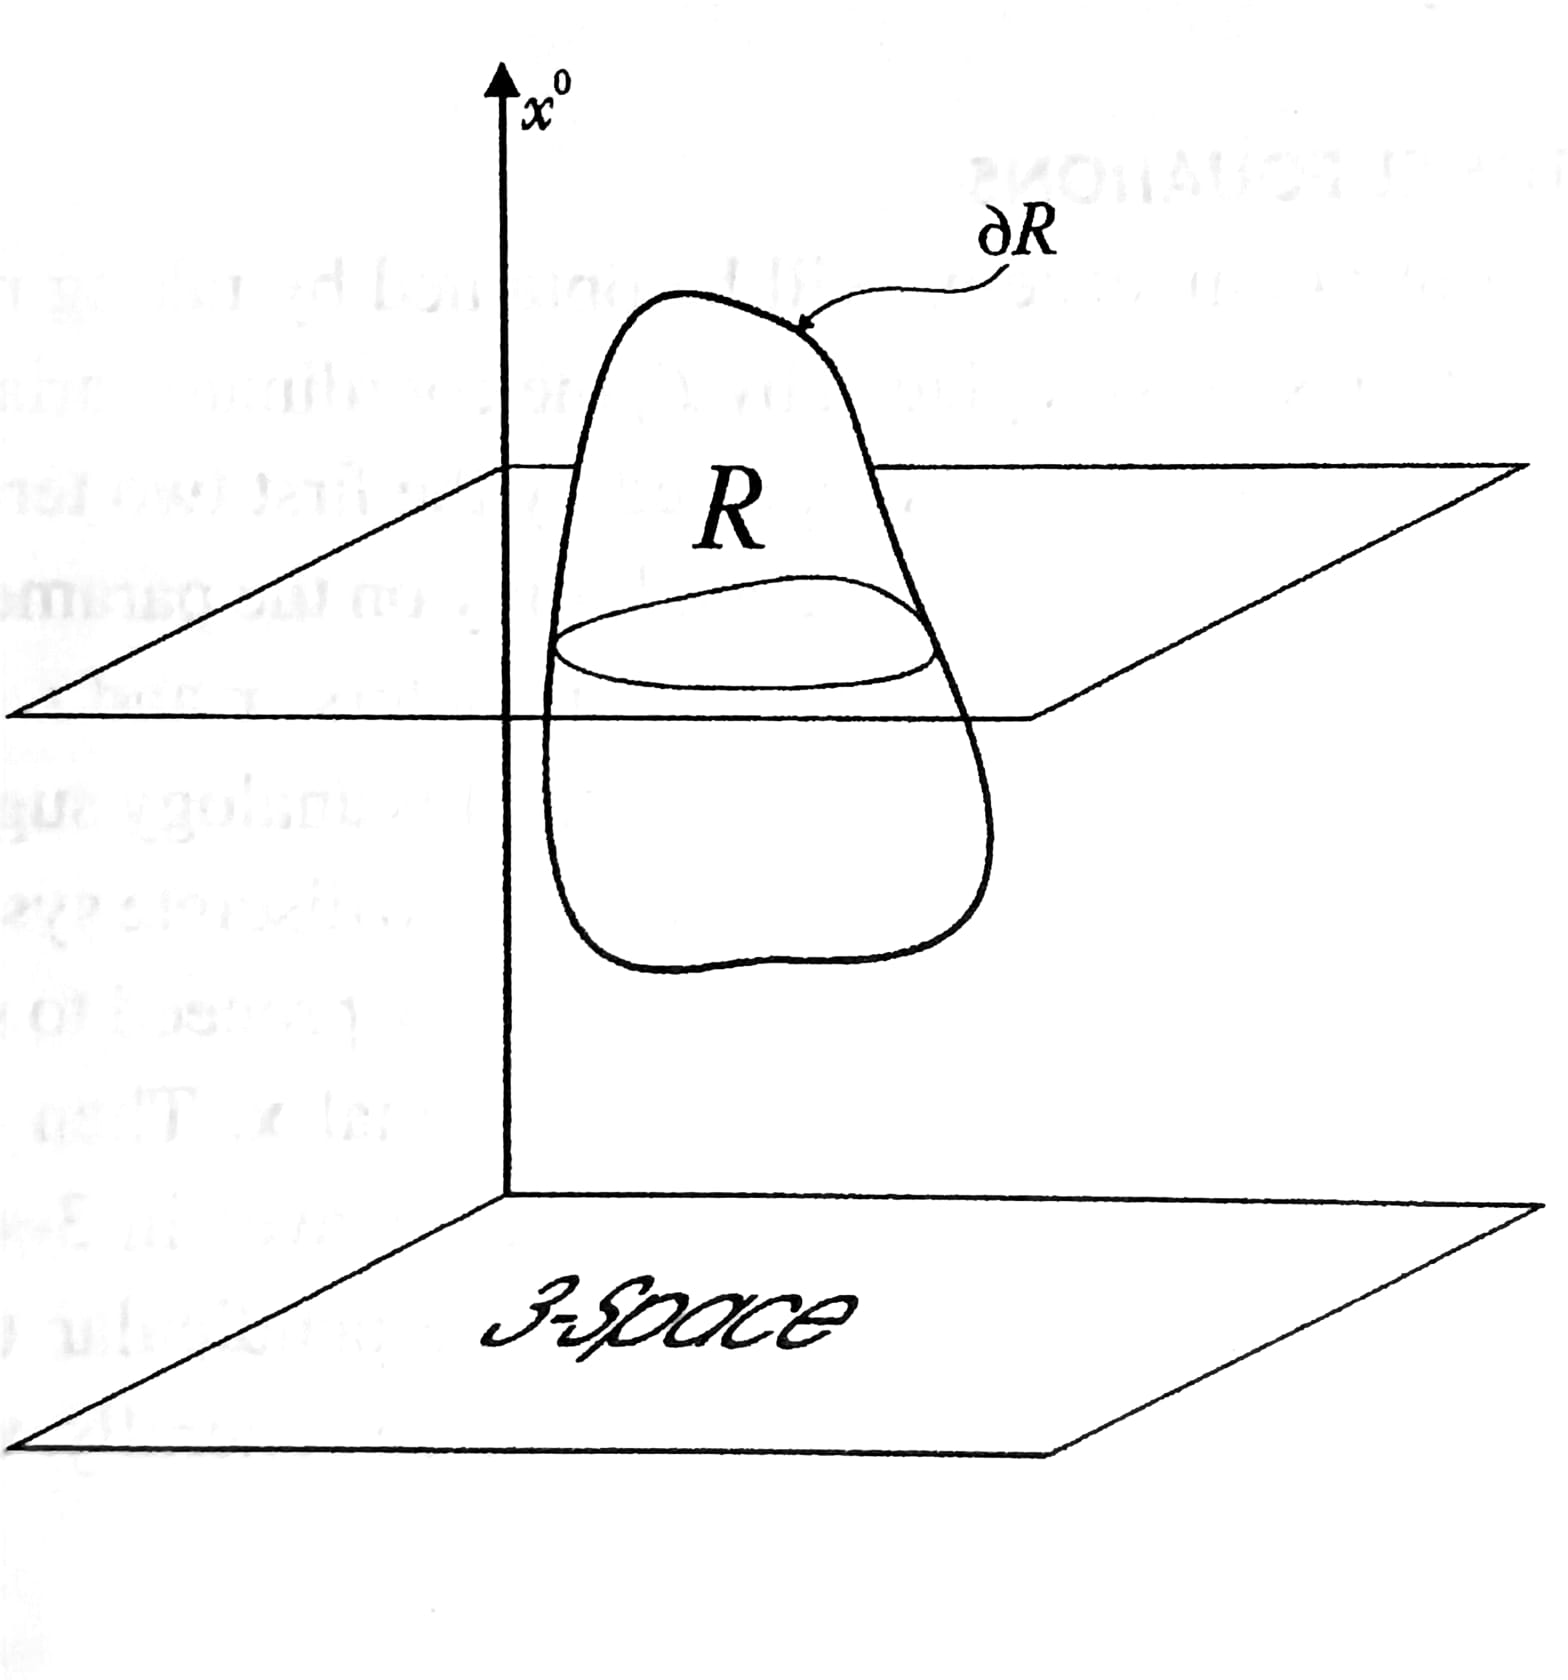
\includegraphics{4-D_REGION.jpg}
  \caption[]{Espacio de Minkowski de 4 dimensiones}
  \labfig{fig:mink}
\end{marginfigure}

Definimos $$K^\mu = \frac{\partial \mathcal{L}}{\partial (\partial_\mu \phi)} \delta \phi \sim \partial_\mu \phi$$. Ahora, aplicando el teorema de la divergencia:
$$
\int_V d^4x \partial_\mu K^\mu = \int_{\Sigma_2}^{\Sigma_1} d\Sigma_\mu K^\mu
$$

Con $\Sigma^\mu$ el cuadrivector perpendicular a la hipersuperficie (ver en \reffig{fig:mink}).

Entonces, el flujo de $K^\mu$ sobre la superficie se anula en toda la frontera de Minkowski:
$$
\delta S = \int d^4x \left( \frac{\partial \mathcal{L}}{\partial \phi} - \partial_\mu \frac{\partial \mathcal{L}}{\partial (\partial_\mu \phi)} \right) \delta \phi \approx 0 \quad \forall \delta \phi \rightarrow
$$

Obteniendo:
$$
\frac{\partial \mathcal{L}}{\partial \phi} - \partial_\mu \frac{\partial \mathcal{L}}{\partial (\partial_\mu \phi)} = 0
$$

\subsubsection{Las ecuaciones de Euler-Lagrange}

Para una acción $S'$ tal que su diferencia con $S$ sea de la forma: $S' = S + \int d^4x f(x)\delta V(\phi) \rightarrow \delta S' = \delta S + \int d^4x \delta V(\phi) = \delta S$: Si la diferencia entre acciones $S$ y $S'$ es la cuadridivergencia de un campo vectorial, entonces ambas tienen las mismas ecuaciones del movimiento.
\subsection{Formalismo Hamiltoniano}

Una vez descrito el formalismo Lagrangiano, podemos ir al formalismo Hamiltoniano de forma análoga a como lo haciamos en mecánica clásica, para ello definimos el \textit{Momento canónico generalizado} como 

\[\Pi(x)=\pdv{\mathcal{L}}{\partial(\partial_{0}\phi_{i})}\text{ con }\partial_{0}\phi_{i}= \dot{\phi}\]

De forma que el Hamiltoniano queda definido como 

\[\mathcal{H}=\Pi\dot{\phi_{i}}-\mathcal{L}\]

\subsection{Ejemplos}

\begin{example}[Campo escalar real sin interacción]
  $$
  \mathcal{L}_0 = \frac{1}{2} \partial_\mu \phi \partial^\mu \phi - \frac{1}{2} m^2 \phi^2 = \mathcal{L}_0 (\phi, \partial_\mu \phi)
  $$
  A partir de estos lagrangianos y las ecuaciones de Euler-Lagrange es posible obtener la ecuación de Klein-Gordon:
  $$
  \frac{\partial \mathcal{L}}{\partial \phi} = -m^2 \phi
  $$
  $$
  \partial_\mu \frac{\partial \mathcal{L}}{\partial (\partial_\mu \phi)} = \Box \phi \quad \Rightarrow \quad (\Box + m^2) \phi = 0
  $$

\end{example}
\begin{example}[Campo escalar real con interacción]

  $$
    \mathcal{L} = \frac{1}{2} \partial_\mu \phi \partial^\mu \phi - \frac{1}{2} m^2 \phi^2 - V(\phi) = \mathcal{L}_0 - V(\phi)
    $$
    La ecuación de Klein-Gordon obtenida a partir de este lagrangiano sería:
    $$
    (\Box + m^2) \phi = -V'(\phi) = \frac{\partial V(\phi)}{\partial \phi}
    $$
  
\end{example}
\begin{example}[Campo complejo]
  El campo es de la forma: $\phi = \phi_1 + i \phi_2 \in \mathbb{C}$, con $\phi_i \in \mathbb{R}$, $i = 1, 2$. El lagrangiano sería:
  $$
  \mathcal{L} = -\partial_\mu \phi^* \partial^\mu \phi - m^2 |\phi|^2 - V(|\phi|^2)
  $$

  Donde hemos considerado que $\phi_1$ y $\phi_2$ dependen de la misma masa. Para el cálculo de K-G es equivalente trabajar con $\phi_1$ y $\phi_2$ como campos independientes que trabajar con $\phi$ y $\phi^*$:
  $$
  (\Box + m^2) \phi^* = -\frac{\partial V}{\partial |\phi|^2} \phi^*
  $$
  $$
  (\Box + m^2) \phi = -\frac{\partial V}{\partial |\phi|^2} \phi
  $$
\end{example}
\begin{example}[Campo electromagnético con potencial]
  $$
    \mathcal{L} = -\frac{1}{4} F^{\mu\nu} F_{\mu\nu} - A_\mu J^\mu
    $$

    Con $F^{\mu\nu}$ el tensor de campo electromagnético, definido como:
    $$
    F^{\mu\nu} = \partial^\mu A^\nu - \partial^\nu A^\mu
    $$

    El término $-\frac{1}{4} F_{\mu\nu} F^{\mu\nu}$ es el campo electromagnético libre, mientras que el término $A_\mu J^\mu$ se refiere a la interacción. Con las ecuaciones de Euler-Lagrange para este lagrangiano podemos obtener el segundo par de ecuaciones de Maxwell.
\end{example}
\begin{example}[Partícula en campo electromagnético]
  $$
    \mathcal{L} = -\frac{1}{4} F_{\mu\nu} F^{\mu\nu} + (D_\mu \phi)^* (D^\mu \phi) - m^2 |\phi|^2
    $$

    Recordando que, para una partícula en un campo electromagnético, $D_\mu$ toma la forma $D_\mu = \partial_\mu + iq A_\mu$, podemos reescribir el lagrangiano como:
    $$
    \mathcal{L} = -\frac{1}{4} F_{\mu\nu} F^{\mu\nu} + |(\partial_\mu + iq A_\mu) \phi|^2 - m^2 |\phi|^2
    $$

    donde:
    $$
    J^\mu = iq (\phi^* \partial^\mu \phi - \phi \partial^\mu \phi^*)
    $$

    Es la corriente conservada asociada a la simetría de gauge. Así, las ecuaciones de movimiento para los campos complejos en presencia de un campo electromagnético toman la forma:
    $$
    (\Box + m^2) \phi = -2iq \partial^\mu A_\mu \phi - 2iq A_\mu \partial^\mu \phi + q^2 A_\mu A^\mu \phi
    $$
    $$
    (\Box + m^2) \phi^* = 2iq \partial^\mu A_\mu \phi^* + 2iq A_\mu \partial^\mu \phi^* + q^2 A_\mu A^\mu \phi^*
    $$

    Lo que implica que $\phi^*$ se comporta como $\phi$, pero con una carga opuesta, $-q$.
\end{example}
\begin{example}[Lagrangiano de Dirac]
  $$
  \mathcal{L} = \frac{i}{2} (\bar{\psi} \gamma^\mu \partial_\mu \psi - \partial_\mu \bar{\psi} \gamma^\mu \psi) - m \bar{\psi} \psi
  $$

  Con $\psi$ el cuadriespinor de Dirac (ver L.D.) y $\bar{\psi} = \psi^\dagger \gamma^0$ el adjunto de Dirac. Introduciendo la notación slash de nuevo:
  $$
  \mathcal{L} = \bar{\psi} (\slashed{\partial} - m) \psi
  $$
\end{example}
\begin{example}[Cuadriespinor de Dirac en campo electromagnético]
  $$
    \mathcal{L} = -\frac{1}{4} F^{\mu\nu} F_{\mu\nu} + \bar{\psi} (i \slashed{D} - m) \psi - A_\mu J^\mu
    $$
    En esta expresión:

\begin{itemize}

    \item $-\frac{1}{4} F_{\mu\nu} F^{\mu\nu}$ representa el lagrangiano libre del campo electromagnético.
    
    \item $\bar{\psi} (i \slashed{\partial} - m) \psi$ es el lagrangiano libre del campo de Dirac.
    
    \item $A_\mu J^\mu$ es el término de interacción entre el cuadriespinor de Dirac y el campo electromagnético.

\end{itemize}
Esta expresión es conocida como el \textbf{lagrangiano de Maxwell-Dirac}. Si la corriente conservada está dada por:
$$
J^\mu = q \bar{\psi} \gamma^\mu \psi
$$

Entonces las ecuaciones de movimiento son:
$$
\partial_\mu F^{\mu\nu} = J^\nu, \quad i\slashed{D} \psi = m \psi
$$

Donde se verifica que la corriente es conservada $(\partial_\mu J^\mu = 0)$.
\end{example}
\section{Teorema de Noether}

El teorema de Noether es una herramienta fundamental en el estudio de la dinámica de los cuerpos, por lo que también es relevante ver como es su formalismo en teoría de campos.
\subsection{Corrientes}
En mecánica Lagrangiana decíamos que una coordenada era una constante del movimiento cuando su momento canónico conjugado era constante, es decir,
$$\dot{p}_{q^a}=0\rightarrow p_{q^a}=const \qquad q^a \text{ es cíclica}$$
esto implicaba que podíamos cambiar $q$ por una coordenada $q'$ parametrizada por un parámetro $\epsilon$ de tal forma que $L$ es invariante. 

El teorema de Noether relaciona las simetrías en la integral de acción con leyes de conservación. Considerando una transformación infinitesimal de las coordenadas:

$$
x'^\mu = x^\mu + \delta x^\mu
$$

$$
\phi(x) = \phi(x) + \delta \phi(x)
$$

%\begin{definition}[Variación tilda]… \end{definition}
Además usaremos la propiedad de conmutación
$$
 \left[ \delta, \partial_\mu \right] = 0
$$

La acción de la transformación infinitesimal es de la forma :

\begin{equation}
\tilde{\delta} S=\int d^4 x^{\prime} \mathcal{L}^{\prime}\left(x^{\prime}\right)-\int d^4 x \mathcal{L}(x)
\end{equation}

El jacobiano para la primera integral al cambiarse la base $(x')$ será:

\begin{equation}
d x^{\prime}=d^4 x^{\prime}=\left\|\frac{\partial x^{\prime \mu}}{\partial x^\nu}\right\| d^4 x=\operatorname{det}\left(\delta^\mu{ }_\nu+\partial_\nu \delta x^\mu\right) d^4 x
\end{equation}

Para resolver esta ecuación, usamos que $\det{e^M} = e^{\text{tr}M}$, por lo que, haciendo un desarrollo en potencias, el determinante queda en primera corrección: $\det(1+M) = 1+\langle M \rangle +\mathcal{O}(M^2)$. Así:

\begin{equation}
d x^{\prime}=\left(1+\operatorname{tr} \partial_\nu \delta x^\mu\right) d x=\left(1+\partial_\mu \delta x^\mu\right) d x \rightarrow d x^{\prime} \mathcal{L}=d x\left(1+\partial_\mu \delta x^\mu\right) \mathcal{L}
\end{equation}
Sustituyendo de nuevo en la transformación general:

\begin{equation}
\begin{aligned}
\tilde{\delta} S & =\int d x(\overbrace{\mathcal{L}^{\prime}\left(x^{\prime}\right)-\mathcal{L}(x)}^{\tilde{\delta} \mathcal{L}}+\partial_\mu \delta x^\mu \mathcal{L}(x))=\int d x\left(\delta \mathcal{L}+\delta x^\mu \partial_\mu \mathcal{L}+\partial_\mu \delta x^\mu \mathcal{L}\right)= \\
& =\int d x\left(\delta \mathcal{L}+\partial_\mu\left(\delta x^\mu \mathcal{L}\right)\right)=\int d x\left(\frac{\partial \mathcal{L}}{\partial \phi} \delta \phi+\frac{\partial \mathcal{L}}{\partial\left(\partial_\mu \phi\right.} \delta \partial_\mu \phi+\partial_\mu\left(\delta x^\mu \mathcal{L}\right)\right)= \\
& =\int d x\left[\left(\frac{\partial \mathcal{L}}{\partial \phi}-\partial_\mu \frac{\partial \mathcal{L}}{\partial\left(\partial_\mu \phi\right)}\right)_{\text {EMov }} \delta \phi+\partial_\mu\left(\frac{\partial \mathcal{L}}{\partial\left(\partial_\mu \phi\right)} \delta \phi\right)+\partial_\mu\left(\delta x^\mu \mathcal{L}\right)\right]
\end{aligned}
\end{equation}

Se dice que tenemos una transformación de simetría si $ \delta S = 0 $, es decir, tendrá las mismas ecuaciones de movimiento tras la transformación. Decimos que $ \delta x^\mu $ y $ \delta \phi $ son simetrías del sistema si conducen a las mismas ecuaciones del movimiento, es decir, a $ \delta S = 0 $. Tomando el caso en el que tenemos transformación de simetría, la integral se debe anular:

$$
\left( \frac{\partial \mathcal{L}}{\partial \phi} - \partial_\mu \left( \frac{\partial \mathcal{L}}{\partial (\partial_\mu \phi)} \right) \right)_{\text{EMov}} \delta \phi + \partial_\mu \left( \frac{\partial \mathcal{L}}{\partial (\partial_\mu \phi)} \delta \phi + \delta x^\mu \mathcal{L} \right) = 0
$$

Definimos así el cuadrivector \textit{corriente Noether}:

$$
J^\mu = \left( - \frac{\partial \mathcal{L}}{\partial (\partial_\mu \phi)} \delta \phi \right) - \left( \delta x^\mu \mathcal{L} \right)
$$

Así, la condición para la simetría se simplifica:

$$
\partial_\mu J^\mu = \left( \frac{\partial \mathcal{L}}{\partial \phi} - \partial_\mu \frac{\partial \mathcal{L}}{\partial (\partial_\mu \phi)} \right)_{\text{EMov}} \delta \phi
$$

Es decir, la condición de simetría se reduce a:

$$
\partial_\mu J^\mu = 0
$$

$ J^\mu $ es una cantidad conservada. El conjunto de las transformaciones de simetría forman grupo, que denotaremos por $\{J^\mu_a\}$, tales que $J^\mu=\epsilon J^\mu_a$, es decir,  $J^\mu_a$ es el generador del grupo.

% Sea $ \delta x^\mu = \epsilon^a A^\mu_a $, con $ \epsilon^a \ll 1 $; y sea $ \delta \phi_i = \epsilon^a F_{ai}(\phi, \partial \phi) \rightarrow \delta \phi_i = \epsilon^a (F_{ai} - A^\mu_a \partial_\mu \phi_i) $, con $ a = 1, \ldots, n $, siendo $ n $ la dimensión del grupo. Con esto, podemos escribir $ J^\mu $ como:

% $$
% J^\mu = \epsilon J^\mu_a, \quad \text{con} \quad J^\mu_a = \frac{\partial \mathcal{L}}{\partial (\partial_\mu \phi_i)} (A^\nu_a \partial_\nu \phi_i - F_{ai}) - A^\mu_a \mathcal{L}
% $$

% Que sigue verificando $ \partial_\mu J^\mu_a = 0 $. 
\subsection{Cargas}
Podemos definir también las \textit{cargas de Noether} asociadas a las transformaciones de simetría:
$$
Q_a = \int dx J^0_a \quad \Rightarrow \quad \frac{dQ_a}{dt} = 0
$$

Consideremos un cambio en la corriente: $ J^\mu_a \rightarrow J^\mu_a = J^\mu_a + \partial_\nu A^{\mu \nu}_a $ Con $ A^{\mu \nu}_a $ anti-simétrico. Calculando $ \partial_\mu J^\mu_a $:

$$
\partial_\mu J^\mu_a = \partial_\mu J^\mu_a + \partial_\nu \partial_\mu A^{\mu \nu}_a = 0
$$
Esta ambigüedad está relacionada con la de la lagrangiana en una derivada total.
\section{Transformaciones de simetria espacio-temporales}
Dependiendo de la forma de las transformaciones (3.56), podemos distinguir distintos tipos de simetrías:

Simetrías globales: los parámetros $\theta^{a}$ son independientes de las coordenadas; las simetrías globales son un caso especial de las simetrías locales.

Simetrías locales: los parámetros $\theta^{a}(x)$ dependen de las coordenadas
Simetrías internas: $X_{a}^{\mu}(x)=0$, es decir, las coordenadas no cambian.
Simetrías espacio-temporales: $X_{a}^{\mu}(x) \neq 0$, es decir, involucran cambios en las coordenadas.
\subsection{Traslaciones}
El ejemplo más sencillo es la simetría bajo traslaciones, dadas en el caso infinitesimal por

\begin{aligned}
x^{\prime \mu} & =x^{\mu}+\theta^{\mu} \\
\phi_{i}^{\prime}\left(x^{\prime}\right) & =\phi_{i}(x) \tag{3.63}
\end{aligned}

En este caso, el índice $a=1, \ldots, 4$ podemos sustituirlo por un índice griego $v$, de forma que

\begin{aligned}
X_{v}^{\mu} & =\delta^{\mu}{ }_{v} \\
Y_{i, v} & =0 \tag{3.64}
\end{aligned}

La corriente conservada se lee en este caso

\begin{equation*}
\theta^{\mu v}=\frac{\partial \mathscr{L}}{\partial\left(\partial_{\mu} \phi_{i}\right)} \partial^{v} \phi_{i}-\eta^{\mu v} \mathscr{L} . \tag{3.65}
\end{equation*}
donde hemos usado $\theta^{\mu \nu}=\eta^{\nu \rho} \theta_{\rho}^{\mu}$. Esta corriente conservada se conoce como tensor energíamomento.

La conservación de la corriente implica

\begin{equation*}
\partial_{\mu} \theta^{\mu v}\left(\phi^{c l}\right)=0 \tag{3.66}
\end{equation*}
y las cargas son
\begin{equation*}
P^{v} \equiv \int d^{3} x \theta^{0 v}\left(\phi^{c l}\right) \tag{3.67}
\end{equation*}
que es el cuadrimomento del campo.
Nótese que $\theta^{\mu \nu}$ no es simétrico en sus índices. Sin embargo, podemos construir un tensor simétrico

\begin{equation*}
T^{\mu v}=\theta^{\mu v}+\partial_{\rho} A^{\rho \mu v} \tag{3.68}
\end{equation*}
con $A$ un tensor antisimétrico en los índices $\rho, \mu$ elegido adecuadamente. Precisamente debido a la antisimetría de $A$, el nuevo tensor también es conservado
$$
\partial_{\mu} T^{\mu v}=\partial_{\mu} \partial_{\rho} A^{\rho \mu v}=0
$$

Para $\mu=0$ tenemos $\partial_{\rho} A^{\rho 0 v}=\partial_{i} A^{i 0 v}$ que es una divergencia espacial y por tanto no cambia las cargas conservadas en (3.67). En otras palabras, $\theta^{\mu v}$ y $T^{\mu v}$ son físicamente equivalentes y podemos trabajar con cualquiera de ellos. $T^{\mu v}$ se conoce como tensor energía-momento simetrizado de Belinfante-Rosenfeld.
\subsection{Transformaciones de Lorentz}
Consideremos ahora el caso en el que la acción es invariante bajo transformaciones de Lorentz dadas anteriormente en (3.6) y (3.31)

\[\begin{aligned}
  x^{\prime \mu} & =x^{\mu}+\omega_{v}^{\mu} x^{v} \\
  \phi_{i}^{\prime}\left(x^{\prime}\right) & =\phi_{i}(x)-\frac{i}{2} \omega_{\mu v}\left[S^{\mu v}\right]_{i}^{j} \phi_{j}(x) \tag{3.69}
  \end{aligned}\]

de forma que ahora el índice $a$ se convierte en un par de índices griegos $\nu , \rho$

\begin{gather*}
X^{\mu v \rho}=\frac{1}{2}\left(\eta^{\mu v} x^{\rho}-\eta^{\mu \rho} x^{v}\right) \\
Y_{i}^{v \rho}=-\frac{i}{2}\left[S^{v \rho}\right]_{i}^{j}{ }_{i} \phi_{j}(x) \tag{3.70}
\end{gather*}
donde los generadores $\left[S^{v \rho}\right]_{i}^{j}$ se escribirán en la representación correspondiente a los campos $\phi_{i}$.

La correspondiente corriente de Noether será

\begin{equation*}
j^{\mu}=\left[\frac{\partial \mathscr{L}}{\partial\left(\partial_{\mu} \phi_{i}\right)}\left(-\frac{i}{2}\left[S^{v \rho}\right]_{i}^{j} \phi_{j}(x)-X^{\lambda v \rho}(x) \partial_{\lambda} \phi_{i}(x)\right)+\mathscr{L} X^{\mu v \rho}(x)\right] \omega_{v \rho} \tag{3.71}
\end{equation*}

Esta corriente se puede escribir como

\begin{equation*}
j^{\mu}=\frac{1}{2} M^{\mu \nu \rho} \omega_{v \rho} \tag{3.72}
\end{equation*}
donde $M^{\mu v \rho}$ se puede escribir en función del tensor energía-momento como

\begin{equation*}
M^{\mu v \rho}=x^{v} \theta^{\mu \rho}-x^{\rho} \theta^{\mu v}+S^{\mu v \rho} \tag{3.73}
\end{equation*}
con

\begin{equation*}
S^{\mu v \rho}=-i \frac{\partial \mathscr{L}}{\partial\left(\partial_{\mu} \phi_{i}\right)}\left[S^{v \rho}\right]_{i}^{j} \phi_{j} \tag{3.74}
\end{equation*}

La conservación de la corriente implica

\begin{equation*}
\partial_{\mu} M^{\mu v \rho}=0 \tag{3.75}
\end{equation*}

Por tanto, tenemos 6 corrientes conservadas, $M^{\mu v \rho}$ una por cada uno de los 6 parámetros independientes de la transformación de Lorentz $\omega_{v \rho}$. Nótese que por construcción $M^{\mu v \rho}$ es antisimétrico en ( $v \rho$ ). Las correspondientes cargas conservadas son:

\begin{equation*}
M^{v \rho}=\int d^{3} x M^{0 v \rho}=\int d^{3} x\left(x^{v} p^{\rho}-x^{\rho} p^{v}+S^{0 v \rho}\right) \tag{3.76}
\end{equation*}
$\operatorname{con} p^{v}=\theta^{0 v}$ la densidad de cuadrimomento.
Nótese que las 3 cargas conservadas $M^{i j}$, asociadas a las rotaciones, proporcionan el momento angular del campo como

\begin{equation*}
J^{i}=\frac{1}{2} \epsilon^{i j k} M^{j k} \tag{3.77}
\end{equation*}
que como vemos tienen la contribución del momento angular orbital ( $\left.x^{i} p^{j}-x^{j} p^{i}\right)$ y de spin $S^{0 i j}$. Las $M^{0 i}$ corresponderían a las 3 cargas conservadas asociadas a los boosts.\sidenote{La interpretación física de estas cargas conservados no es tan directa y puede verse que corresponden a la posición del centro de momentos del campo en el instante $t=0$.}